\subsection{Análisis de datos}

Tras la recopilación de datos, se efectuará un análisis descriptivo para inspeccionar la distribución de los resultados tanto en la guía de programación como en la primera evaluación. Adicionalmente, se realizará un análisis de correlación entre las variables previamente mencionadas con el fin de discernir relaciones y patrones significativos.

\subsubsection{Descripción de la base de datos}

A continuación, se detalla la estructura de la base de datos:

\begin{table}[H]
    \centering
    \caption{Descripción de variables}
    \begin{tabular}{lp{0.6\linewidth}}
        \toprule
        \textbf{Variable}        & \textbf{Descripción}                                          \\
        \midrule
        sol1                     & Nota en la primera evaluación (rango 0-7)                     \\
        exitosos                 & Cantidad de respuestas correctas en la guía                   \\
        fallidos                 & Número de intentos en la guía                                 \\
        hito1 hito2              & Expectativas de aprendizaje del curso (conjunto de preguntas) \\
        programa                 & Programa académico del estudiante                             \\
        Columnas e0 hasta la e52 & Resultados de la guía (1: correcto, 0: incorrecto)            \\
        \bottomrule
    \end{tabular}
    \label{tab:variables}
\end{table}

Las columnas descritas son esenciales para nuestro análisis, ya que nos facilitan la exploración de la relación entre la resolución de la guía de programación, el rendimiento académico en la primera evaluación y el programa académico del estudiante (véase Tabla \ref{tab:variables}).

\subsubsection{Variable Objetivo}

El propósito principal de esta investigación es determinar la influencia de la resolución de la guía en el desempeño de la evaluación del curso. Por ello, se propone la variable \textit{sol1} como variable objetivo. Dado su carácter cuantitativo, se recomienda añadir una columna denominada \textit{aprobado}, de naturaleza binaria. En esta columna, se asignará el valor 1 a las notas que oscilen entre 4.0 y 7.0, y el valor 0 a las notas inferiores, denotando la condición de reprobado. Esta transformación se ilustra en el siguiente fragmento de código:

\begin{lstlisting}[language=Python, caption=Tratamiento de la Variable Objetivo ,label=lst:trat_varObjetivo]
    # Creación de la columna 'aprobado' y población de la misma.
    df["aprobado"] = df.apply(lambda x: functions.set_in_aprobado_nota(x["sol1"]), axis=1)
\end{lstlisting}

\subsubsection{Descripción del DataFrame}

La Tabla \ref{tab:descripcion_dataframe} ofrece un resumen del DataFrame, detallando las columnas, la cantidad de valores no nulos y los tipos de datos asociados. Esta descripción brinda una perspectiva general de la estructura y características del DataFrame.

\begin{table}[H]
    \centering
    \caption{Descripción del DataFrame}
    \begin{tabular}{lll}
        \hline
        \textbf{Columna} & \textbf{Non-Null Count} & \textbf{Dtype} \\
        \hline
        hito1            & 839 non-null            & float64        \\
        hito2            & 839 non-null            & float64        \\
        exitosos         & 839 non-null            & int64          \\
        fallidos         & 839 non-null            & int64          \\
        sol1             & 839 non-null            & float64        \\
        aprobado         & 839 non-null            & int64          \\
        e0 - e52         & 839 non-null            & int64          \\
        \hline
    \end{tabular}%
    \label{tab:descripcion_dataframe}%
\end{table}%

Como se observa en la Tabla \ref{tab:descripcion_dataframe}, cada columna cuenta con 839 valores no nulos y se especifica el tipo de dato correspondiente. Estos detalles son cruciales para entender la composición y propiedades del DataFrame en estudio.

\subsubsection{Estadísticas de la variable objetivo}

Dentro del análisis de datos, es esencial conocer las características estadísticas de las variables numéricas. En este contexto, se ha examinado la variable \textit{sol1}, recopilando estadísticas como el recuento, la media, la desviación estándar, los cuartiles y el sesgo. Estos valores ofrecen una visión sobre la distribución y tendencia central de la variable.

\begin{table}[H]
    \centering
    \caption{Estadísticas de la variable objetivo}
    \begin{tabular}{ll}
        \hline
        \textbf{Medida}    & \textbf{Valor}       \\
        \hline
        Count              & 839.000000           \\
        Mean               & 3.642789             \\
        Standard Deviation & 1.832625             \\
        Minimum            & 1.000000             \\
        25\% Percentile    & 2.200000             \\
        50\% Percentile    & 3.700000             \\
        75\% Percentile    & 5.100000             \\
        Maximum            & 7.000000             \\
        Skewness           & 0.033079652062595215 \\
        \hline
    \end{tabular}%
    \label{tab:estadistica_variable_sol1}%
\end{table}%

La Tabla \ref{tab:estadistica_variable_sol1} revela que la variable \textit{sol1} tiene una media cercana a 3.6 y una desviación estándar alrededor de 1.83. La distribución de los datos muestra un ligero sesgo positivo con un valor de aproximadamente 0.03. Estos resultados nos permiten entender la variabilidad y forma de la distribución de la variable \textit{sol1}.

\subsubsection{Coeficiente de asimetría de la variable objetivo}

El coeficiente de asimetría es una métrica que brinda información sobre la asimetría de una distribución de datos. Para los datos analizados, se ha obtenido un coeficiente de asimetría de aproximadamente 3.31\%. Este valor señala una ligera asimetría positiva en la distribución.

\begin{table}[H]
    \centering
    \caption{Coeficiente de asimetría}
    \begin{tabular}{ll}
        \hline
        \textbf{Coeficiente de asimetría}      & \textbf{Valor}       \\
        \hline
        Coeficiente de asimetría               & 0.033079652062595215 \\
        Coeficiente de asimetría en porcentaje & 3.31\%               \\
        \hline
    \end{tabular}%
    \label{tab:skewness}%
\end{table}%

La Tabla \ref{tab:skewness} muestra un coeficiente de asimetría de 0.033079652062595215, lo que indica una ligera asimetría hacia la derecha. Esto sugiere que hay una cola derecha más extensa en comparación con la cola izquierda de la distribución. En términos porcentuales, esta asimetría representa aproximadamente el 3.31\% del rango total de la distribución.

\subsubsection{Coeficiente de Variación de la variable objetivo}

El coeficiente de variación es una métrica que refleja la dispersión relativa de una variable respecto a su media. Facilita la evaluación de la variabilidad de los datos en relación con su valor medio. Se calcula dividiendo la desviación estándar entre la media y se expresa en porcentaje.

\begin{table}[H]
    \centering
    \caption{Coeficiente de Variación}
    \begin{tabular}{ll}
        \hline
        \textbf{Medida}                        & \textbf{Valor}     \\
        \hline
        Coeficiente de Variación               & 0.5027829289053924 \\
        \hline
        Coeficiente de Variación en Porcentaje & 50.28\%            \\
        \hline
    \end{tabular}%
    \label{tab:coef_variacion}%
\end{table}%

La Tabla \ref{tab:coef_variacion} muestra el coeficiente de variación calculado para los datos analizados. Este coeficiente es de aproximadamente 0.5027, lo que indica una alta dispersión relativa respecto a la media. Esto se confirma con el coeficiente de variación en porcentaje, que es del 50.28\%. Estos resultados subrayan la variabilidad de los datos en el conjunto analizado.

\subsubsection{Amplitud de la variable objetivo}

La amplitud es una métrica que refleja la variabilidad o dispersión de los datos. Permite evaluar la diferencia entre el valor máximo y mínimo de una variable, proporcionando información sobre la extensión de los datos en el conjunto.

\begin{table}[H]
    \centering
    \caption{Amplitud}
    \begin{tabular}{ll}
        \hline
        \textbf{Medida} & \textbf{Valor}     \\
        \hline
        Amplitud        & 0.5600809456082252 \\
        \hline
    \end{tabular}%
    \label{tab:amplitud}%
\end{table}%

La Tabla \ref{tab:amplitud} muestra la amplitud calculada para los datos analizados. La amplitud es de aproximadamente 0.56\%, lo que indica la diferencia entre el valor máximo y mínimo de la variable. Esta métrica nos proporciona una idea de la extensión de los datos en el conjunto analizado.

\subsubsection{Tabla de Frecuencias de la variable objetivo}

Utilizando los datos de la Tabla \ref{tab:skewness} y la Tabla \ref{tab:amplitud}, se ha elaborado una tabla de frecuencias que refleja la distribución de los datos en intervalos. Los intervalos se definen en función de la amplitud y el valor máximo de los datos.

\begin{table}[H]
    \centering
    \caption{Tabla de Frecuencias}
    \begin{tabular}{lllll}
        \hline
        \textbf{Intervalo} & \textbf{f\_i} & \textbf{F\_i} & \textbf{h\_i} & \textbf{H\_i} \\
        \hline
        (0.0, 0.56]        & 0             & 0             & 0.000000      & 0.000000      \\
        (0.56, 1.12]       & 152           & 152           & 0.181168      & 0.181168      \\
        (1.12, 1.68]       & 21            & 173           & 0.025030      & 0.206198      \\
        (1.68, 2.24]       & 66            & 239           & 0.078665      & 0.284863      \\
        (2.24, 2.8]        & 79            & 318           & 0.094160      & 0.379023      \\
        (2.8, 3.36]        & 34            & 352           & 0.040524      & 0.419547      \\
        (3.36, 3.92]       & 103           & 455           & 0.122765      & 0.542312      \\
        (3.92, 4.48]       & 76            & 531           & 0.090584      & 0.632896      \\
        (4.48, 5.04]       & 87            & 618           & 0.103695      & 0.736591      \\
        (5.04, 5.6]        & 81            & 699           & 0.096544      & 0.833135      \\
        (5.6, 6.16]        & 53            & 752           & 0.063170      & 0.896305      \\
        (6.16, 6.72]       & 57            & 809           & 0.067938      & 0.964243      \\
        \hline
    \end{tabular}%
    \label{tab:tabla_frecuencias}%
\end{table}%

La Tabla \ref{tab:tabla_frecuencias} presenta la tabla de frecuencias que muestra la cantidad de datos en cada intervalo, el total acumulado de datos hasta ese intervalo, la frecuencia relativa del intervalo y la frecuencia relativa acumulada. Esta tabla nos permite visualizar la distribución de los datos y su acumulación en cada intervalo.

El intervalo más relevante es (3.36, 3.92], ya que contiene la mayor frecuencia (103) y la mayor acumulación (455). Esto indica que la mayoría de los datos se encuentran en este rango.

A continuación, se presenta una tabla con información adicional:

\begin{table}[H]
    \centering
    \caption{Información Adicional}
    \begin{tabular}{llll}
        \hline
        \textbf{Mediana} & \textbf{Intervalo de la mediana} & \textbf{Máximo} & \textbf{Intervalo del máximo} \\
        \hline
        3.7              & $f_i$ 103.000000                 & 7.0             & $f_i$ 57.000000               \\
                         & $F_i$ 455.000000                 &                 & $F_i$ 809.000000              \\
                         & $h_i$ 0.122765                   &                 & $h_i$ 0.067938                \\
                         & $H_i$ 0.542312                   &                 & $H_i$ 0.964243                \\
        \hline
    \end{tabular}%
    \label{tab:informacion_adicional}%
\end{table}%

La Tabla \ref{tab:informacion_adicional} muestra la mediana de los datos y el intervalo en el que se encuentra. También se indica el valor máximo y el intervalo correspondiente.

\subsubsection{Histograma con curva de densidad de la variable objetivo}

El histograma con curva de densidad es una herramienta visual que permite comprender la distribución de los valores de la variable \textit{sol1}.

\begin{figure}[H]
    \centering
    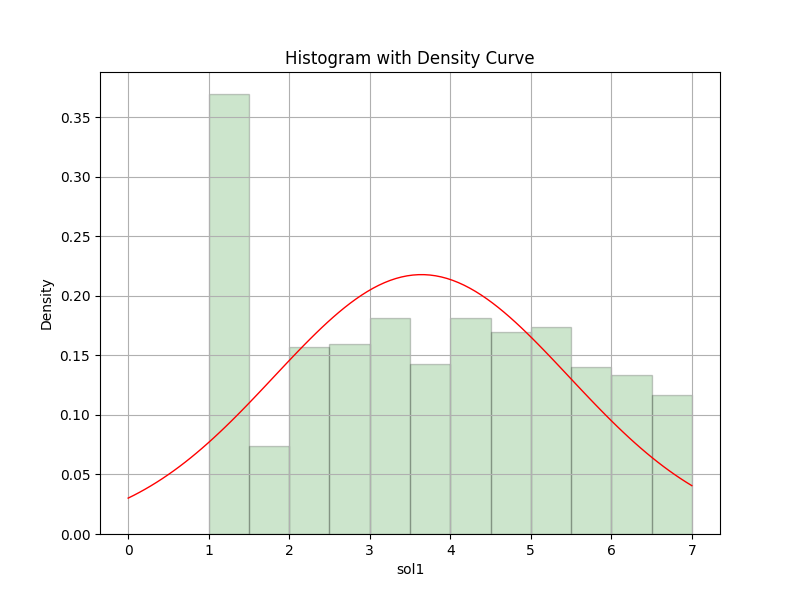
\includegraphics[width=4.06111in,height=2.68611in]{img/histogramaConCurvaDeDensidad.png}
    \caption{Histograma con Curva de Densidad}
    \label{fig:hist_density}%
\end{figure}%

La Figura \ref{fig:hist_density} muestra el histograma con curva de densidad correspondiente a los datos analizados. En el eje Y, se presentan los valores de densidad, mientras que en el eje X, se muestran las notas obtenidas en \textit{sol1}. La mayor concentración de datos se encuentra alrededor del valor 0.35 en el eje Y, lo que indica que la mayoría de las observaciones tienen una nota baja en \textit{sol1}. La curva de densidad, representada en rojo, alcanza su punto más alto entre las notas 3 y 4 en el eje X. Esta curva suavizada muestra la forma general de la distribución de los valores de \textit{sol1}. A medida que las notas aumentan, la densidad disminuye gradualmente.

\subsubsection{Identificación de valores atípicos de la variable objetivo}

La detección de valores atípicos es esencial en el análisis de datos para identificar observaciones que se desvían significativamente de la tendencia general. Estos valores pueden tener un impacto significativo y requerir un análisis más detallado.

A continuación, se muestra una tabla con los valores atípicos identificados mediante el método del Z-score:

\begin{table}[H]
    \centering
    \caption{Valores Atípicos}
    \begin{tabular}{ccccccc}
        \hline
        \textbf{hito1} & \textbf{hito2} & \textbf{exitosos} & \textbf{fallidos} & \textbf{programa} & \textbf{sol1} & \textbf{aprobado} \\
        21.0           & 6.0            & 17                & 14                & UNAB11500         & 1.0           & 0                 \\
        2.0            & 2.0            & 4                 & 27                & UNAB12210         & 1.0           & 0                 \\
        4.0            & 4.0            & 6                 & 41                & UNAB12510         & 1.5           & 0                 \\
        0.0            & 0.0            & 0                 & 47                & UNAB12100         & 1.6           & 0                 \\
        10.0           & 6.0            & 9                 & 38                & UNAB11500         & 1.6           & 0                 \\
        12.0           & 0.0            & 9                 & 38                & UNAB12210         & 2.4           & 0                 \\
        42.0           & 12.0           & 26                & 37                & UNAB21500         & 2.5           & 0                 \\
        32.0           & 32.0           & 26                & 5                 & UNAB11500         & 3.4           & 0                 \\
        9.0            & 0.0            & 7                 & 40                & UNAB11500         & 4.3           & 1                 \\
        38.0           & 6.0            & 28                & 35                & UNAB12210         & 4.4           & 1                 \\
        32.0           & 32.0           & 26                & 5                 & UNAB12210         & 4.6           & 1                 \\
        18.0           & 2.0            & 11                & 20                & UNAB12210         & 4.6           & 1                 \\
        32.0           & 14.0           & 21                & 10                & UNAB12210         & 5.9           & 1                 \\
        13.0           & 25.0           & 16                & 15                & UNAB22115         & 7.0           & 1                 \\
        7.0            & 0.0            & 5                 & 42                & UNAB12100         & 7.0           & 1                 \\
        \hline
    \end{tabular}%
    \label{tab:valores_atipicos}%
\end{table}%

Observando los valores atípicos en la tabla \ref{tab:valores_atipicos}, podemos notar que algunas observaciones difieren significativamente en al menos una de las variables. \say{exitosos} representa las respuestas correctas de la guía, \say{fallidos} indica la cantidad de errores para lograr los \say{exitosos}, \say{programa} se refiere a la carrera a la cual pertenece. \say{sol1} se refiere a la nota obtenida en la solemne, \say{aprobado} se refiere si la nota de solemen es mayor mayor o igual a 4 el alumno es aprobado(columna agregada por medio de script). Estos valores atípicos pueden ser de interés para un análisis más detallado, ya que podrían indicar situaciones excepcionales o errores en la recolección de datos.